\documentclass{article}

% NeurIPS 2026 template. Upload neurips_2026.sty from the official template next to this file
% (Overleaf: "NeurIPS 2026" gallery template). Use [final] for the camera-ready, non-anonymous report.
\usepackage[final]{neurips_2026}

\usepackage[utf8]{inputenc}
\usepackage[T1]{fontenc}
\usepackage{hyperref}
\usepackage{url}
\usepackage{booktabs}
\usepackage{amsfonts}
\usepackage{amsmath}
\usepackage{nicefrac}
\usepackage{microtype}
\usepackage{xcolor}
\usepackage{graphicx}
\usepackage{tikz}
\usetikzlibrary{arrows.meta,positioning}
\graphicspath{{figures/}}

\title{Evidence-Constrained Probabilistic Prediction of AI Response Outcomes\\
with Leave-One-Benchmark-Out Model Selection and a Gated Code-Revision Agent}

\author{%
  Saifuddin Abdullah\thanks{AI engineer and developer with more than twenty years of experience in international organisations and agencies, including WHO, RTI International, Management Systems International (DFAT--AusAID), FHI 360, NIPA Korea, Aligner and Outlier. Codabench user \texttt{syehsyoh}.}\\
  Independent AI engineer\\
  \texttt{syehsaifuddin@gmail.com}
}

\begin{document}

\maketitle

\begin{abstract}
We describe our entry to the NeurIPS 2026 Predictive AI Evaluation Competition (PAIEC), which asks a program to predict whether an AI system answers a benchmark item correctly, given subject and item attributes and a small budget of revealed outcomes. Our predictor is an evidence-constrained, Bayesian-inspired model that is deterministic given its inputs when run without API credentials: de-confounded subject priors fitted on the public \texttt{measurement-db} release, a zero-shot item-ease regressor on dual sentence embeddings, a three-regime Beta--Binomial mixture posterior for the revealed labels followed by heuristic peer-pooling and kernel-ridge corrections. Our selected submission scored 0.127586 Brier ALC on the hosted formative evaluation. Because the platform resamples the hidden subset for every submission, we select among candidate predictors with a leakage-free leave-one-benchmark-out (LOBO) simulator built on the public data. It shows that our predictor beats the organizers' baselines by 0.012 Brier ALC, and it also locates the remaining weaknesses: budget-0 predictions are worse than a constant 0.5, the first revealed label adds almost nothing, and at 31 labels the predictor does no better than a constant equal to the pair's pass rate. We release the predictor, the simulator, a QA gate, and a slot-constrained code-revision agent (Qwen2.5-Coder) whose proposals are accepted only on paired LOBO evidence.
\end{abstract}

\section{Introduction}

PAIEC~\cite{paiec} evaluates a submitted program \texttt{predict(input, labeled)} that returns $P(\text{correct})$ for a subject--item pair, at label budgets $n\in\{0,1,3,7,15,31\}$ per subject--benchmark pair. The metric is the normalised area under the Brier learning curve on a $\log_2(n+1)$ axis,
\[
\text{Brier ALC} = 0.1\,B_0 + 0.2\,(B_1+B_3+B_7+B_{15}) + 0.1\,B_{31},
\]
averaged with equal weight over subject--benchmark pairs. Hidden benchmarks are disjoint from the public training benchmarks, so the task is a benchmark-level cold start.

Our contribution is a methodology rather than a single model. (i) A leakage-free local leave-one-benchmark-out (LOBO) protocol that approximates the evaluator, including its acquisition interface and nested budgets, and scores every candidate on identical pairs so that differences are paired (Section~\ref{sec:eval}). (ii) A deterministic shrinkage predictor (Section~\ref{sec:method}) that beats the organizers' empirical-mean and smoothed-empirical-Bayes baselines~\cite{baselines} under that protocol, together with diagnostics that locate where it fails. (iii) A revision of the predictor derived from those diagnostics (Section~\ref{sec:v400}), and a development loop in which an open-weights code-revision agent proposes constrained edits that a QA gate accepts only on paired LOBO evidence (Section~\ref{sec:agent}). We state negative results where we found them.

\section{Data}
\label{sec:data}

\paragraph{Training sources.} We used only the public PAIEC training release of \texttt{aims-foundations/measurement-db}~\cite{mdb} (revision \texttt{54074453}), restricted to the eight benchmarks bundled in our submission: afrimedqa, agentdojo, ai2d\_test, hle, matharena, mathvista\_mini, mmbench\_v11 and mmlupro (200 items each; 19--263 subjects; 1.5k--62k responses). No data outside the benchmark inventory was used. Table~\ref{tab:data} summarises the release. In the release we used, the \texttt{hle} items carry only an identifier in the \texttt{content} field, so they contribute to subject priors but carry no usable text (see Section~\ref{sec:items}).

\begin{table}[t]
\caption{Public training data used (measurement-db, PAIEC subset).}
\label{tab:data}
\centering\small
\begin{tabular}{lrrrr}
\toprule
Benchmark & Subjects & Items & Responses & Mean pass rate \\
\midrule
afrimedqa & 30 & 200 & 3{,}192 & 0.62 \\
agentdojo & 29 & 200 & 11{,}594 & 0.32 \\
ai2d\_test & 254 & 200 & 49{,}936 & 0.75 \\
hle & 19 & 200 & 1{,}517 & 0.27 \\
matharena & 97 & 200 & 34{,}960 & 0.62 \\
mathvista\_mini & 263 & 200 & 55{,}230 & 0.28 \\
mmbench\_v11 & 251 & 200 & 62{,}467 & 0.81 \\
mmlupro & 48 & 200 & 8{,}534 & 0.52 \\
\bottomrule
\end{tabular}
\end{table}

\paragraph{Formative feedback.} Codabench returns, per submission, a table of Brier ALC and ECE for each evaluated subject--benchmark pair under permanent anonymous identifiers. We parsed 38 such logs (328 pair rows, 7 hidden benchmarks, 151 subjects) and used them only in aggregate, to locate where the loss concentrates by budget and benchmark; we did not attempt to identify the benchmarks or subjects behind the anonymous identifiers.

\paragraph{Pretrained models.} The predictor bundles \texttt{sentence-transformers/all-MiniLM-L6-v2}~\cite{minilm} and \texttt{BAAI/bge-small-en-v1.5}~\cite{bge} (declared in \texttt{models.txt}). At budget 0 it may make up to three calls to an approved inference API (\texttt{nvidia/nemotron-3-super-120b-a12b}) through the organizers' Bayesian Linguistic Evaluator agent to obtain a subject--benchmark group prior; the calls are capped at 25 seconds in total and the predictor degrades gracefully to the database prior when no credentials are present. The released archive contains no credentials.

\section{Method}
\label{sec:method}

The submitted predictor (internal name v153) is a single file \texttt{model.py} with fitted artifacts in \texttt{data/}. Figure~\ref{fig:pipeline} shows the flow of one prediction; a glossary of terms is given in Appendix~\ref{app:glossary}. All quantities below are deterministic given the inputs.

\begin{figure}[t]
\centering
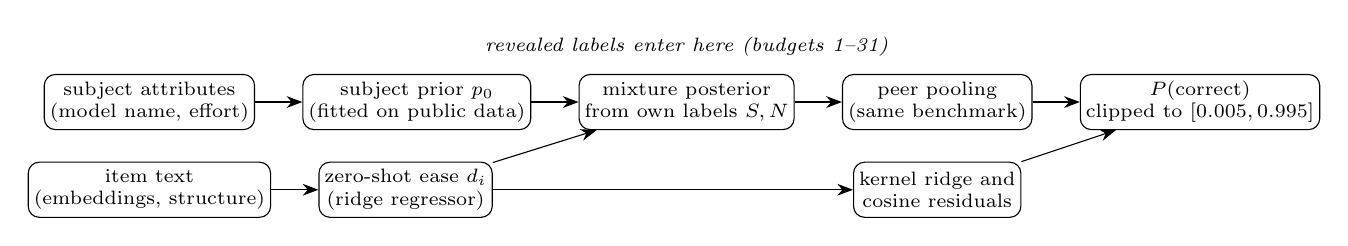
\begin{tikzpicture}[node distance=4mm and 6mm, every node/.style={font=\scriptsize}, box/.style={draw, rounded corners, align=center, minimum height=7mm, inner sep=2pt}, >={Stealth[length=2mm]}]
\node[box] (subj) {subject attributes\\(model name, effort)};
\node[box, right=of subj] (prior) {subject prior $p_0$\\(fitted on public data)};
\node[box, right=of prior] (mix) {mixture posterior\\from own labels $S,N$};
\node[box, right=of mix] (peer) {peer pooling\\(same benchmark)};
\node[box, right=of peer] (out) {$P(\text{correct})$\\clipped to $[0.005,0.995]$};
\node[box, below=of subj] (item) {item text\\(embeddings, structure)};
\node[box, right=of item] (ease) {zero-shot ease $d_i$\\(ridge regressor)};
\node[box, below=of peer] (kr) {kernel ridge and\\cosine residuals};
\draw[->] (subj) -- (prior); \draw[->] (prior) -- (mix); \draw[->] (mix) -- (peer); \draw[->] (peer) -- (out);
\draw[->] (item) -- (ease); \draw[->] (ease) -- (mix); \draw[->] (ease) -- (kr); \draw[->] (kr) -- (out);
\node[above=1mm of mix, font=\scriptsize\itshape] {revealed labels enter here (budgets 1--31)};
\end{tikzpicture}
\caption{One prediction: the subject prior and the zero-shot item ease give the budget-0 estimate; revealed labels update the mixture posterior; peers and item-level residuals correct it.}
\label{fig:pipeline}
\end{figure} Only the mixture step of Section~\ref{sec:posterior} is a posterior in the strict sense; the later peer, kernel-ridge and envelope steps are heuristic corrections whose constants were set during development, and the final output is not the posterior of a single generative model.

\subsection{Subject priors}
For each subject $s$ we fit, per training benchmark, an item-adjusted ability $\theta_{s,b}$ by alternating subject and item fixed effects on the response matrix (40 iterations, ridge $2$ or $14$ depending on the number of items). We aggregate across benchmarks into a general ability $\delta^{\text{gen}}_s$ and a frontier-reasoning ability $\delta^{\text{front}}_s$ (matharena and hle are treated as frontier), store per-benchmark deltas, and resolve subject names at prediction time through a canonicalisation of model names (vendor prefixes, dates, aliases). The frontier/general split uses fixed offsets chosen by inspection of the public data (for example $+0.48$ for non-reasoning models on matharena) rather than estimated effects, which we state plainly because the word ``de-confounded'' in our code should not be read as a causal identification. Unknown subjects fall back to an architecture heuristic keyed on model family and reasoning effort. The priors are keyed on the model name and reasoning effort only; the harness and harness version that the competition includes in its definition of a subject are ignored, so two subjects that differ only in harness receive the same prior (Section~\ref{sec:limits}). At prediction time the general and frontier abilities are mixed with a weight that starts at 0.22 for the frontier component and is adapted from the cosine similarity between the running embedding centroid of the target benchmark and the centroids of the training benchmarks, and, once labels exist, from the observed pass rate of the benchmark (lower pass rates raise the frontier weight). The budget-0 prior is $p_0=\text{clip}(0.449+0.20\,(p_{\text{db}}-0.5),\,0.379,\,0.489)$, where $p_{\text{db}}$ combines the subject delta and mean.

\subsection{Item features and zero-shot ease}
\label{sec:items}
Each item text is embedded with MiniLM (384-d) and bge-small (384-d) and concatenated with 13 structural features (length, digits, math symbols, code keywords, multiple-choice markers), giving a 781-d vector. A linear ridge regressor fitted on the eight benchmarks maps pool-centred features to an item ease $d_i$ and a second linear term that is multiplied by the subject ability ($d_i \leftarrow d_i + 0.38\,\text{disc}_i\,\theta_s$). This is a linear surrogate for the difficulty and discrimination parameters of item response theory~\cite{lord}; no logistic item model is fitted, and the ease is added on the probability scale rather than the logit scale, which is why the predictor needs output clipping and the damping envelope of Section~\ref{sec:peer}. The pool centre for a hidden benchmark is the running mean of the items seen so far, shrunk toward the global mean. Because the \texttt{hle} rows of the release contain identifier strings rather than text, one eighth of the regressor's training rows are effectively noise; we kept the fitted artifact unchanged for the selected submission and list this under limitations.

\subsection{Estimate from revealed labels}
\label{sec:posterior}
With $S$ successes in $N$ revealed outcomes of the subject on the target benchmark, the base estimate is a three-regime Beta--Binomial mixture posterior (near-zero, mid-hard and saturated regimes with pseudo-counts $(0.38,6.80)$, $(3.10,5.10)$ and $(6.20,2.80)$), with regime weights shifted by the prior and by peers. When $0<S<N$ the successes are debiased by the mean ease of the sampled items ($S-0.265\,N\,\bar d$); the correction is not applied at $S=0$ or $S=N$, so the estimate is discontinuous at those boundaries, a heuristic choice we did not validate separately. For $0<S<N$ and $N\le 3$ the estimate is blended toward the prior with weight $0.34$ ($N=1$) or $0.10$ ($N\le3$).

\subsection{Peer pooling and kernel ridge}
\label{sec:peer}
Other subjects evaluated on the same anonymous benchmark contribute a peer mean adjusted by the ability difference $\theta_s-\theta_{s'}$, scaled by a Bernoulli-variance factor $\text{clip}(4.2\,\hat p(1-\hat p),0.35,1.05)$ (the derivative of the logistic link, rescaled); where the subject and a peer have labelled the same item (rare at small budgets) the observed difference replaces part of the prior difference. If a peer has labelled the target item itself, its outcome, shifted by the calibrated difference, is blended into the final prediction with a weight that grows with the number of such peers (capped at 0.56). The peer mean shifts the prior ($0.45\,(\bar y_{\text{peer}}-0.386)\,N_p/(N_p+2)$) and is blended into the base estimate with weight $(N_p/(N_p+3.5))\cdot 1.84/(N+1.84)$. When at least two labelled items exist, a pool-centred quadratic cosine kernel ridge ($K=0.7S+0.3S^2+5.5I$, output clipped to $\pm0.26$) adds an item-level residual, and a cosine-similarity transfer from the subject's own labelled items adds a second residual; both are multiplied by a damping envelope $\text{clip}(\hat p(1-\hat p)/0.06,\,0.15,\,1)$ that suppresses item effects near 0 and 1. Outputs are clipped to $[0.005,0.995]$. A legacy branch returns $0.99$ or $0.01$ when the subject's own revealed labels contain the target item itself; under the evaluator's disjoint acquisition and evaluation pools this branch cannot fire, and it is retained only for interface compatibility.

\subsection{Acquisition}
\texttt{labeling.py} selects labels by deterministic uniform hashing with a complementary tilt toward items not yet labelled by peers on the same benchmark. Because peer items are themselves drawn uniformly, the tilted subset and its complement have the same expected item difficulty by design, so the per-subject sample mean stays unbiased while the union of items labelled across peers grows; we did not re-measure the coverage gain in the simulator. The policy is not an active-learning policy: it does not use the current prediction or its uncertainty to choose informative items, although budgets 1 and 3 carry 40\% of the metric weight. We leave uncertainty- or representativeness-based acquisition, which the interface supports, as the most obvious untested lever.

\subsection{Budget-0 revision}
\label{sec:b0}
LOBO (Section~\ref{sec:eval}) showed that the hard cap at $0.495$ makes budget-0 predictions worse than a constant 0.5. The revised zero-label branch is $\text{clip}(c + s\,(m_s-0.5) + e\,d_i,\,0.02,\,0.98)$ with $m_s$ the subject prior mean, selected on all 905 LOBO pairs over a $3\times5\times5$ grid; we ship $c=0.50$, $s=0.5$, $e=1.0$ as the robust choice ($c=0.55$ is marginally better on the public benchmarks, which are easier on average than the hidden ones appear to be).

\subsection{Revision driven by the LOBO diagnostics: online two-way shrinkage (v400)}
\label{sec:v400}
The diagnostics of Section~\ref{sec:results} show that v153 barely uses its first revealed labels. One structural cause is visible in the code: a subject's labels on \emph{other} benchmarks, which the evaluator reveals in the same \texttt{labeled} list, are used only as a fallback when the subject has no label on the target benchmark, and peers are used only on the target benchmark. The revision fits, at every call, an additive model on all revealed labels,
\[
y_{s,b} \approx \mu + a_s + b_b,
\]
by alternating shrunken means with pseudo-counts $k_s=k_b=3$ ($\mu$ shrunk toward the subject prior with $k_\mu=4$), and blends the resulting estimate for the target pair into the base estimate with a weight that decreases with the number of own labels (profiles $(0.6,0.5,0.3,0.15)$, $(0.4,0.3,0.2,0.1)$ and $(0.8,0.6,0.4,0.2)$ for $N\le1$, $N\le3$, $N\le7$ and $N>7$). The subject key includes harness and harness version, partially addressing the subject-definition mismatch of Section~\ref{sec:method}. Because the original simulator draws only pairs from one benchmark, it cannot exercise cross-benchmark pooling; Section~\ref{sec:eval} describes the context-pair extension used to evaluate v400. The result (Table~\ref{tab:v400}) is negative: the revision is reported here as a tested hypothesis, not as part of the shipped predictor.

\subsection{A logistic item-response estimator at test time (v402)}
\label{sec:v402}
To move from the linear surrogate toward the measurement models the organizers work with, v402 adds a one-parameter logistic estimator fitted at every call on the revealed labels: $P(y_{s,i}=1)=\sigma(\theta_s+\beta_b+\kappa\,d_i)$, with subject ability $\theta_s$ given a Gaussian prior centred at $\mathrm{logit}(p_0)$, benchmark difficulty $\beta_b$ a Gaussian prior centred at 0, item ease $d_i$ taken from the zero-shot regressor and scaled by $\kappa$, and peers' labels entering through their own $\theta_{s'}$ priors. The posterior mode is found by a few damped Newton steps, the prediction for the target item is $\sigma(\hat\theta_s+\hat\beta_b+\kappa\,d_{\text{target}})$, and it is blended into the base estimate with the same budget-dependent weights as v400. Unlike v400, the model is additive on the logit scale and uses item ease inside the likelihood, which is the form item response theory prescribes. Results are reported in Table~\ref{tab:v402}.

\section{Evaluation protocol}
\label{sec:eval}

\subsection{Why a local protocol}
Each formative evaluation samples a new subset of the hidden pool (at most 1{,}000 subject--item pairs; in our logs 8--9 subject--benchmark pairs from 7 hidden benchmarks), and per-pair Brier ALC differs strongly by benchmark (Figure~\ref{fig:hidden}). Two submissions are therefore scored on different samples, and the final evaluation uses a common subset for all teams. For model selection we rely on a local protocol in which every candidate is scored on identical pairs, and we use the formative tables only as paired, per-benchmark observations under the permanent anonymous identifiers.

\begin{figure}[t]
\centering
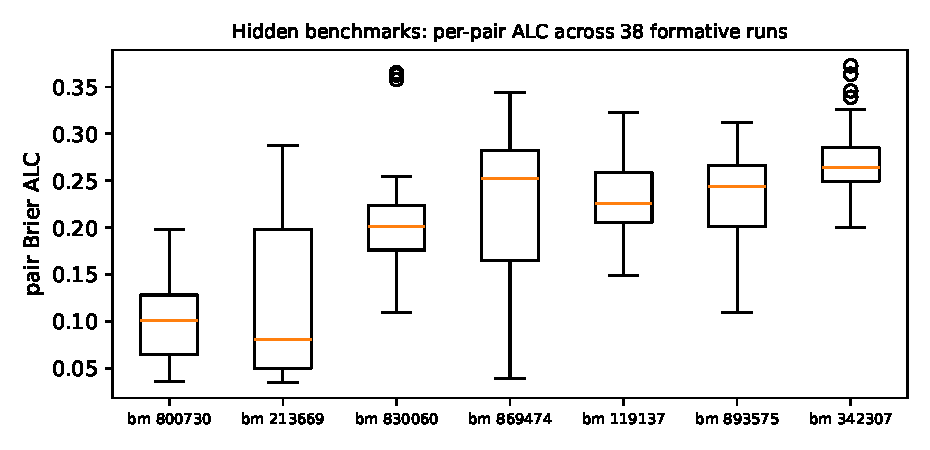
\includegraphics[width=0.85\linewidth]{hidden_benchmarks.pdf}
\caption{Per-pair Brier ALC of the seven hidden benchmarks across 38 formative runs of successive development versions (v9--v59), keyed by the platform's anonymous identifiers, which we do not interpret. The spread therefore mixes benchmark difficulty with model changes; the ordering of benchmarks is stable across versions. Two benchmarks have near-zero pass rates and are solved by one label; the other five carry the loss.}
\label{fig:hidden}
\end{figure}

\subsection{Leave-one-benchmark-out simulator}
We built a local simulator that mirrors the evaluator: for each held-out public benchmark, the fitted artifacts are patched to remove that benchmark (its per-benchmark subject deltas are dropped and re-averaged, subjects known only from it become unseen, and the item-ease ridge, feature mean and centroids are refit without it); the benchmark identifier is anonymised; items of each eligible subject ($\ge 80$ items) are split 50/50 into acquisition and evaluation pools by a fixed hash; labels are acquired through our \texttt{labeling.py} via the organizers' streaming acquisition hook with nested budgets; and Brier ALC is computed per pair with the official weights. Draws of 1--3 pairs share a benchmark so peer labels are present, although fewer peers than in the hosted evaluation, where several subjects per hidden benchmark appear in one run. Seven text folds (hle excluded for lack of text) with 16 pairs each give 112 pairs that are identical across variants, so differences are paired. Network calls are disabled. Budget-0 variants are additionally scored on all 905 eligible pairs, since budget-0 predictions do not depend on labels. Because pairs within a draw share peer labels and pairs within a fold share patched artifacts, we report standard errors both over pairs and over the seven folds.

\paragraph{Context pairs.} On Codabench, \texttt{labeled} also contains labels of the same subject on other hidden benchmarks. To evaluate predictors that pool across benchmarks, the extended protocol adds to each draw up to two unscored pairs of the same subjects on other public benchmarks (never hle); their labels enter \texttt{labeled} with their own anonymised benchmark identifiers, and only the held-out pairs are scored. Context benchmarks are training benchmarks for the fitted priors, so this extension is an approximation that favours any predictor using the priors; the comparison between v153 and v400 under it is nevertheless paired and leakage-free with respect to the scored benchmark.

\section{Results}
\label{sec:results}

\begin{table}[t]
\caption{LOBO results on 112 paired pairs (7 public folds). Differences are paired against v153; SE$_p$ is over pairs, SE$_f$ over the seven folds, and ``folds'' counts folds whose mean improves.}
\label{tab:lobo}
\centering\small
\begin{tabular}{lrrrrrrrrrrr}
\toprule
Variant & ALC & $\Delta$ & SE$_p$ & SE$_f$ & folds & $B_0$ & $B_1$ & $B_3$ & $B_7$ & $B_{15}$ & $B_{31}$ \\
\midrule
v153 (submitted) & 0.2220 & -- & -- & -- & -- & 0.2559 & 0.2497 & 0.2225 & 0.2098 & 0.2026 & 0.1947 \\
v153 + budget-0 fix ($c{=}0.50$) & 0.2212 & $-0.0008$ & 0.0003 & 0.0009 & 5/7 & 0.2482 & \multicolumn{5}{l}{identical to v153} \\
v153 + budget-0 fix ($c{=}0.55$) & 0.2209 & $-0.0011$ & 0.0005 & 0.0017 & 5/7 & 0.2448 & \multicolumn{5}{l}{identical to v153} \\
Smoothed empirical Bayes (org.) & 0.2340 & $+0.0120$ & 0.0025 & 0.0043 & 2/7 & 0.2500 & 0.2643 & 0.2453 & 0.2209 & 0.2112 & 0.2071 \\
Empirical mean (org.) & 0.2633 & $+0.0413$ & 0.0039 & 0.0061 & 0/7 & 0.2500 & 0.3868 & 0.2653 & 0.2238 & 0.2118 & 0.2072 \\
\midrule
Oracle: constant at pair pass rate & -- & -- & -- & -- & -- & \multicolumn{6}{l}{0.1942 at every budget (same 112 pairs)} \\
\bottomrule
\end{tabular}
\end{table}

\begin{figure}[t]
\centering
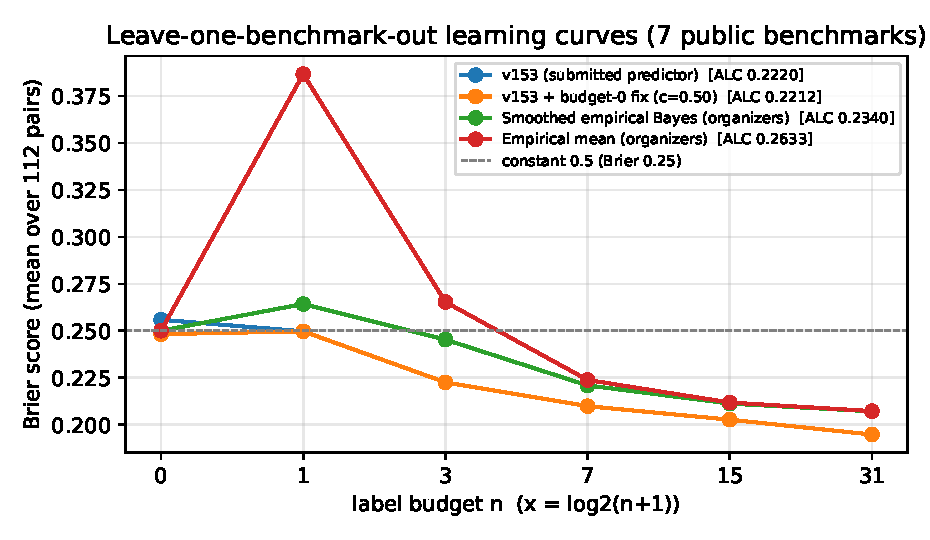
\includegraphics[width=0.9\linewidth]{lobo_curves.pdf}
\caption{LOBO learning curves. The predictor gains from labels only beyond budget 3 and converges to the pair-mean floor by budget 31.}
\label{fig:curves}
\end{figure}

Table~\ref{tab:lobo} and Figure~\ref{fig:curves} summarise the leakage-free comparison. Four observations follow.

\begin{enumerate}
\item \textbf{The predictor beats the official baselines} by 0.012 and 0.041 ALC (pair-level SE 0.0025 and 0.0039; fold-level SE 0.0043 and 0.0061). The budget-0 revision improves 5 of 7 folds but its fold-level SE is of the same size as its effect, so we report it as a small, consistent gain rather than a significant one.
\item \textbf{Budget 0 is worse than predicting 0.5} (0.2559 vs.\ 0.2500), consistent with 0.2546 averaged over 38 earlier formative runs of this model family. The cold-start prior does not transfer across benchmarks. The budget-0 revision of Section~\ref{sec:b0} recovers 0.008--0.011 Brier at budget 0 (0.0008--0.0011 ALC), but the gap to a constant at the true pair pass rate (0.1942) remains the dominant cold-start opportunity.
\item \textbf{The first label adds almost nothing} ($B_1=0.2497$ vs.\ $B_0=0.2559$), although budgets 1 and 3 carry 40\% of the metric weight.
\item \textbf{At 31 labels the predictor equals a constant at the pair pass rate.} On the same 112 pairs, $B_{31}=0.1947$ against an oracle constant of 0.1942 (paired difference $+0.0005$, SE 0.0022; 58 of 112 pairs below the oracle). The item-level terms therefore produce no measurable discrimination on held-out benchmarks at budget 31; the component ablation in Table~\ref{tab:ablation} tests this directly.
\item \textbf{How much evidence is needed.} Measured against the oracle constant, the predictor is within 0.016 Brier of it after 7 labels, within 0.008 after 15, and within 0.001 after 31. For the decision maker of the competition's motivation, this says that about fifteen graded responses per system and benchmark recover most of what is knowable about the pass rate, while the remaining gap, item-level predictability, is not captured by text features alone.
\end{enumerate}

\begin{table}[t]
\caption{Component ablation of v153 on the same 112 LOBO pairs (paired $\Delta$ALC of the ablated model against v153; positive means removing the component hurts, i.e.\ the component helps).}
\label{tab:ablation}
\centering\small
\begin{tabular}{lrrrrr}
\toprule
Ablation & $\Delta$ALC & SE$_p$ & SE$_f$ & folds worse & $\Delta B_{31}$ \\
\midrule
no peer pooling & $+0.0045$ & 0.0013 & 0.0020 & 6/7 & $+0.0044$ \\
no kernel ridge and cosine transfer & $+0.0013$ & 0.0002 & 0.0004 & 7/7 & $+0.0050$ \\
no cosine transfer only & $+0.0002$ & 0.0000 & 0.0001 & 4/7 & $+0.0008$ \\
no IRT envelope term (weight 0.32 $\to$ 0) & $+0.0006$ & 0.0001 & 0.0001 & 7/7 & $+0.0004$ \\
random acquisition instead of \texttt{labeling.py} & $-0.0002$ & 0.0003 & 0.0004 & 4/7 & $-0.0004$ \\
\bottomrule
\end{tabular}
\end{table}

Table~\ref{tab:ablation} separates the components. Peer pooling is the only component with a sizeable effect (0.0045 ALC, 6 of 7 folds). The kernel ridge contributes 0.0013 ALC, concentrated at budgets 7--31 ($+0.0050$ at $B_{31}$), so the item-level terms do add a small amount of discrimination, which refines observation 4 above: they are not useless, but their contribution is an order of magnitude smaller than the gap to a hierarchical pair-rate estimate. The cosine transfer and the IRT envelope are negligible, and our acquisition policy is indistinguishable from random acquisition ($-0.0002$, 4 of 7 folds), so none of the 0.012 advantage over the organizers' baselines comes from acquisition.

\begin{table}[t]
\caption{v400 (budget-0 fix + online two-way shrinkage) against v153 on the same 112 held-out pairs under the context-pair protocol (two unscored same-subject pairs from other public benchmarks per scored pair). Paired $\Delta$ against v153; negative is better.}
\label{tab:v400}
\centering\small
\begin{tabular}{lrrrrrr}
\toprule
Variant & $\Delta$ALC & SE$_p$ & SE$_f$ & folds improved & $\Delta B_1$ & $\Delta B_3$ \\
\midrule
budget-0 fix only ($c{=}0.50$) & $-0.0006$ & 0.0003 & 0.0010 & 5/7 & $-0.0000$ & $-0.0001$ \\
v400a, weights (0.6/0.5/0.3/0.15) & $-0.0000$ & 0.0010 & 0.0019 & 3/7 & $+0.0026$ & $+0.0006$ \\
v400b, weights (0.4/0.3/0.2/0.1) & $-0.0008$ & 0.0008 & 0.0016 & 4/7 & $+0.0001$ & $-0.0003$ \\
v400c, weights (0.8/0.6/0.4/0.2) & $+0.0010$ & 0.0013 & 0.0021 & 2/7 & $+0.0068$ & $+0.0013$ \\
\bottomrule
\end{tabular}
\end{table}

\begin{table}[t]
\caption{v402 (budget-0 fix + logistic item-response estimator) against v153 on the same 112 held-out pairs, context-pair protocol, with calibration diagnostics. Pending: filled from \texttt{localsim/results/calib16\_ctx2}.}
\label{tab:v402}
\centering\small
\begin{tabular}{lrrrrrr}
\toprule
Variant & $\Delta$ALC & SE$_p$ & SE$_f$ & folds & ECE$_1$ & ECE$_{31}$ \\
\midrule
budget-0 fix only & pending & & & & & \\
v402a ($\kappa{=}3,\tau_s{=}2,\tau_b{=}2$, weights 0.4/0.3/0.2/0.1) & pending & & & & & \\
v402b (same, weights 0.6/0.5/0.3/0.15) & pending & & & & & \\
v402c ($\kappa{=}5,\tau_s{=}4,\tau_b{=}1$, weights 0.4/0.3/0.2/0.1) & pending & & & & & \\
\bottomrule
\end{tabular}
\end{table}

\paragraph{Outcome of the v400 revision.} The two-way estimator does not help (Table~\ref{tab:v400}); the plain protocol without context pairs gives the same picture ($\Delta$ALC $+0.0001$, $-0.0006$ and $+0.0011$ for v400a, b and c, pair-level SE 0.0006--0.0011). Its whole effect is confined to budgets 1--3, where a large weight on the pooled estimate makes $B_1$ worse ($+0.0068$ for v400c) and a small weight reproduces the budget-0 fix alone (v400b, $-0.0008$, within one fold-level SE of the fix by itself). We read this as a negative result with two caveats: the context benchmarks are training benchmarks whose subject deltas the priors already encode, so the simulation cannot show the gain that cross-benchmark labels might give for subjects unknown to the priors; and the additive model works on the probability scale with shrunken means rather than a logistic likelihood. Neither caveat justifies shipping v400; the shipped revision is the budget-0 fix alone, and the next candidates are the peer-precision and low-budget-shrinkage edits that the ablation and the agent batch point to.

\paragraph{Hosted results.} Our selected Codabench submission (ID 1020778, v153) scored 0.127586 Brier ALC on its formative evaluation; at the time of writing the public leaderboard showed it second behind 0.117238. Before the local protocol existed we had made 172 scored formative submissions across the generations of Appendix~\ref{app:generations}; since the protocol, candidates are selected locally and hosted submissions serve as paired per-benchmark checks, which we state here as part of a responsible use of the shared evaluation platform. Fourteen budget-0-revised variants (14 IDs between 1031487 and 1031501, listed in Appendix~\ref{app:ids}) were submitted together with byte-identical controls, to obtain paired per-benchmark observations; their results are appended as they arrive. We note the power of such a test in advance: with per-submission variability of the order of 0.03 and 25 submissions per arm, the standard error of a difference between arms is about 0.008, so the hosted evaluation can confirm or refute only effects an order of magnitude larger than the budget-0 fix measured locally. The hosted batch therefore serves as a consistency check per anonymous benchmark, not as the primary evidence.

\section{What produced the result: an inventory of contributing factors}
\label{sec:factors}

This section lists, as completely as we can, what we did and what each step contributed, because the result is the sum of many small, individually verified decisions rather than one idea. Effects quoted are paired LOBO differences on the same 112 pairs unless stated otherwise.

\subsection{The theory the student was taught}
The agent does not learn by gradient; it is instructed. Its knowledge pack (\texttt{qwen\_knowledge\_v2.json}, built by \texttt{build\_qwen\_knowledge\_v2.py}) contains: (i) the conjugate update that underlies the predictor, $\mathbb{E}[\theta\mid S,N]=(S+a)/(N+a+b)$, and the reading of pseudo-counts as prior strength, so that proposals about regimes and shrinkage are phrased in those terms; (ii) the LOBO evidence for every editable slot (budget-0 Brier worse than 0.5; first label adding nothing; peer pooling worth 0.0045 ALC; the item-level terms worth at most 0.0013), with the allowed range and the baseline value of each parameter; (iii) the rule that formative samples are redrawn per submission, so that a baseline may only be justified by paired LOBO evidence and code lineage; (iv) the metric definition and its budget weights; (v) the contract rules on format, ranges, distinctness and forbidden content. A proposal that contradicts this material (for example a justification by a single hosted score) is flagged by the gate rather than accepted.

\subsection{Tooling built around the local model}
Every script below is released. \texttt{sim\_local.py}/\texttt{sim\_worker.py}: the leakage-free LOBO simulator with artifact patching, fixed splits, nested budgets, the organizers' acquisition hook, context pairs and per-worker timeouts. \texttt{b0\_eval\_fold.py}/\texttt{b0\_eval\_driver.py}: the budget-0 evaluation on all 905 eligible pairs and the $3\times5\times5$ grid that selected the budget-0 revision. \texttt{make\_ablations.py}, \texttt{make\_v400.py}, \texttt{make\_v401.py}: deterministic builders of ablation and revision candidates. \texttt{qa\_gate.py}: the seven static gates (compilation, archive layout, credentials and network imports, slot confinement, unique SHA-256 against the batch and all upload ledgers, hidden identifiers, prediction smoke test with a known and an unknown subject) followed by the LOBO verdict. \texttt{strip\_hidden\_ids.py}: comment-only cleanup verified by AST equality. \texttt{paiec\_qwen\_slot\_generator\_70.py} (v1) and \texttt{paiec\_qwen\_param\_generator\_70.py} (v2): the Kaggle T4 kernels in which the student runs locally; v2 renders edits from templates and smoke-tests each candidate before packaging. \texttt{make\_random\_slot\_candidates.py}: the no-LLM control sampler on the same slots. \texttt{autopilot.py}: screening, full-protocol confirmation, decision, staging, upload, feedback and report in one unattended run. \texttt{push\_kernel\_v3.py}: injects the judged proposals and learned rules into the next student run. \texttt{select\_50.py}, \texttt{upload\_batch.py}: staging with 40-character names and quota-aware upload with ledgers.

\subsection{Generational baseline discipline}
\label{sec:generations}
Development proceeded in generations. Each generation is a batch of submissions derived from one baseline; after the batch is scored, the best member becomes the baseline from which the next generation starts, and nothing is ever derived from a non-baseline candidate. Table~\ref{tab:generations} lists the chain: the smoothed empirical-Bayes reference was succeeded by v9, then v41, v44 and v59, and finally v153. v153 then served as the root of every later batch: the concentric single-constant sweeps v156--v271, the apex sweep v272--v321, the budget-0 revision batch v340--v363, both student batches, the ablations, the v400 and v401 revisions and the no-LLM control batch. In total six batches and more than 250 candidates were derived from v153 in the attempt to exceed it, and the generation did not advance because no candidate exceeded it under the gate. Generations before v153 were promoted on hosted formative scores; from v153 onward, promotion requires the full-protocol LOBO gate ($\Delta\text{ALC}\le-0.0005$, $\Delta+2\,\text{SE}<0$, at least 4 of 7 folds), so that the next baseline is selected on identical pairs rather than on resampled hosted draws. The gate enforces lineage mechanically: a candidate's archive layout must match the baseline and its \texttt{model.py} is diffed against the baseline's; the student is told which baseline to use and why, and its own stated justification is recorded and checked. At the time of writing the baseline is v153 with the budget-0 revision, and v401 (budget-0 revision plus the best student mixture-prior proposal) is under evaluation as the first candidate that could advance the generation. One byte-identical control accompanies every upload day so that hosted results can be read as paired per-benchmark differences.

\subsection{Inventory of efforts and their measured contribution}
\begin{itemize}\setlength{\itemsep}{1pt}
\item \emph{(not separately measured)} Item-adjusted, two-factor subject priors fitted by alternating fixed effects on the public release: the cold-start input to every prediction; the nearest comparison is the organizers' empirical mean, which has no priors and is $0.041$ ALC worse.
\item \emph{(measured indirectly)} Three-regime Beta--Binomial mixture with ease-debiased successes and low-budget blending: the base estimate at every budget $\ge1$; the student's best proposals on its pseudo-counts lower $B_1$ by 0.001.
\item \emph{(measured)} Peer pooling with ability-difference correction: $+0.0045$ ALC, the single largest component.
\item \emph{(measured)} Pool-centred kernel ridge: $+0.0013$ ALC, concentrated at budgets 7--31.
\item \emph{(measured)} Cosine transfer and IRT envelope: $+0.0002$ and $+0.0006$ ALC (retained; negligible).
\item \emph{(measured)} Complementary acquisition policy: $-0.0002$ ALC relative to random (no measurable effect; retained for coverage).
\item \emph{(measured)} Budget-0 revision: $-0.0006$ to $-0.0011$ ALC, 5 of 7 folds.
\item \emph{(indirect)} The LOBO protocol itself: it replaced selection on resampled hosted feedback with paired, leakage-free comparison, rejected the v400 hypothesis before upload, and separated the components above.
\item \emph{(process)} QA gate and autopilot: zero invalid archives uploaded since their introduction; nine semantically broken student edits and one hung candidate caught before upload.
\item \emph{(process)} Credential and identifier hygiene: all API keys removed from archives, hidden benchmark identifiers removed from comments with AST-verified equality.
\item \emph{(hosted, different samples)} All 172 scored submissions beat the constant predictor (Brier 0.25), and 30 of them (17.4\%) scored below 0.1686, the hosted score of our own first submission, a smoothed empirical-Bayes predictor built on the organizers' empirical-mean baseline; this reference is ours, not an organizers' leaderboard entry, and hosted scores of different submissions come from different samples. On identical LOBO pairs every v153-family variant we evaluated beats both organizer baselines.
\end{itemize}

\section{Development loop: gated code revision by an open-weights agent}
\label{sec:agent}

Earlier development explored single-constant sweeps of v153 (concentric radii around the prior centres, blend weights, debias slope and damping) evaluated on hosted formative feedback. Because formative samples differ between submissions, we moved candidate selection to the local protocol of Section~\ref{sec:eval} and organised the search as a constrained loop.

\paragraph{Agent.} A code-revision agent proposes one edit at a time to \texttt{model.py} as a \texttt{<CHANGE>} JSON block (\texttt{old}, \texttt{new}, \texttt{hypothesis}, \texttt{params}). Our initial model-selection experiments used API-hosted coders (Gemini 3 Flash through a Kaggle model proxy, NVIDIA-hosted Nemotron and Qwen2.5-Coder-32B, IBM Granite). Rate limits, expiring proxy credentials, retired endpoints and per-call cost made that loop unreliable and expensive, so we moved the agent to a GPU with open-weights Qwen2.5-Coder~\cite{qwen}: Qwen2.5-0.5B-Instruct for local format tests, Qwen2.5-Coder-1.5B-Instruct on a Kaggle T4 for the first batches, and Qwen2.5-Coder-3B-Instruct (fp16, after the 4-bit 7B failed to load) for the slot-based batch reported here. The open-weights choice lets the organizers rerun the loop without API credentials. Contract compliance is modest: within a 50-minute GPU budget the 3B student processed 53 of 69 planned candidates and produced 16 accepted edits (9 at the first attempt), with 37 candidates rejected after three attempts, mostly for empty or malformed \texttt{<CHANGE>} blocks or edits outside the slot (Appendix~\ref{app:ids}). Syntactically valid edits can still be semantically wrong: one accepted budget-0 edit called the subject lookup on \texttt{item.get('subject')}, which is \texttt{None}, and was caught by the prediction smoke test; five others called \texttt{.get('mean')} on the result of the subject lookup without handling subjects absent from the priors, passed the smoke test (whose subject is known) and failed only inside the LOBO evaluation on held-out subjects. All nine budget-0 edits of the batch were rejected for one of these two reasons, which is itself a finding about using small code models for this task. We therefore changed the division of labour in a second version of the loop: the student proposes only parameter values for a slot (a JSON object), the harness renders the edit from tested templates (including a \texttt{None}-safe budget-0 branch), compiles it, and runs \texttt{predict} with a known and an unknown subject at 0, 1 and 2 labels before packaging. In this mode every packaged candidate is structurally valid by construction; whether it improves the predictor remains the LOBO gate's decision. The same slot ranges sampled without a language model (Latin-hypercube, fixed seed) form the control batch against which the student is compared (Appendix~\ref{app:ids}). We have not yet run the control that this design calls for, a parameter sampler on the same slot ranges without a language model; until it exists, the agent should be read as a constrained random-search proposal mechanism whose value over plain sampling is unproven. The agent is given a knowledge pack (all scored submissions, per-benchmark formative tables, LOBO results, slot definitions) and is first asked to choose and justify the baseline on that evidence; the baseline is v153, the best submission in both hosted and LOBO evaluation, and every candidate is derived from its source tree.

\paragraph{Slots and radius.} Edits are confined to five code regions motivated by the LOBO findings: the budget-0 branch, the low-budget shrinkage block, the mixture-prior pseudo-counts, the peer shift, and the IRT envelope. Each slot has explicit parameter ranges; a radius tier ($\pm25\%$, $\pm50\%$, or the full range) is assigned per candidate, and candidates must differ from each other by at least 1\% of a range.

\begin{figure}[t]
\centering
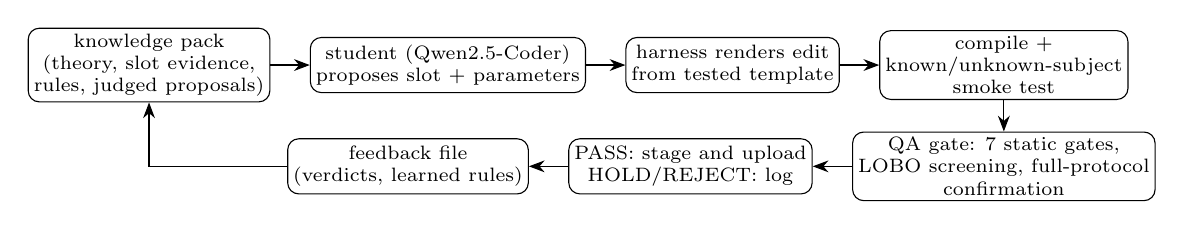
\begin{tikzpicture}[node distance=4mm and 5mm, every node/.style={font=\scriptsize}, box/.style={draw, rounded corners, align=center, minimum height=7mm, inner sep=2pt}, >={Stealth[length=2mm]}]
\node[box] (kp) {knowledge pack\\(theory, slot evidence,\\rules, judged proposals)};
\node[box, right=of kp] (st) {student (Qwen2.5-Coder)\\proposes slot + parameters};
\node[box, right=of st] (rend) {harness renders edit\\from tested template};
\node[box, right=of rend] (smoke) {compile +\\known/unknown-subject\\smoke test};
\node[box, below=of smoke] (gate) {QA gate: 7 static gates,\\LOBO screening, full-protocol\\confirmation};
\node[box, left=of gate] (dec) {PASS: stage and upload\\HOLD/REJECT: log};
\node[box, left=of dec] (fb) {feedback file\\(verdicts, learned rules)};
\draw[->] (kp) -- (st); \draw[->] (st) -- (rend); \draw[->] (rend) -- (smoke); \draw[->] (smoke) -- (gate);
\draw[->] (gate) -- (dec); \draw[->] (dec) -- (fb); \draw[->] (fb) -| (kp);
\end{tikzpicture}
\caption{The gated revision loop. The student never writes code; every packaged candidate is valid by construction, and only the LOBO gate decides what is uploaded. Verdicts feed the next run.}
\label{fig:loop}
\end{figure}

\paragraph{QA gate.} Figure~\ref{fig:loop} shows the loop. A reviewer script enforces: compilation; identical archive layout; no credentials, network imports or hidden identifiers; all changed lines inside the assigned slot; unique SHA-256; a prediction smoke test; and then paired LOBO evaluation against v153 (fast budget-0 evaluation for budget-0-only edits, the full-curve simulator otherwise). A candidate is accepted for upload only if $\Delta\text{ALC}\le-0.0005$, $\Delta+2\,\text{SE}<0$ and at least four of seven folds improve. One byte-identical control per upload day is always included. The whole loop is unattended: a driver script screens every candidate (4 folds, 8 pairs), confirms those within $-0.0003$ ALC of the threshold on the full protocol, stages and uploads the accepted ones, writes a per-slot feedback file (judged proposals and parameter spans that proved indistinguishable from v153) that is injected into the next student run, and produces a report whose only human-facing section lists tool failures.

\section{Limitations}
\label{sec:limits}

\paragraph{Implications for decision makers.} The competition is motivated by organisations that must judge an AI system from a small evaluation. Our results translate into three practical statements: a handful of graded responses is nearly worthless unless it is combined with an informative prior and with results of comparable systems on the same task; about fifteen graded responses per system and task recover most of the knowable pass rate; and predicting which individual items a system will fail, as opposed to how many, is not possible from task text alone with the features we used.

Three limitations concern the scientific framing. The predictor is an engineered shrinkage pipeline: only its mixture step is a posterior, its item-effect surrogate is linear on the probability scale, and about twenty of its constants (Appendix~\ref{app:constants}) have no sensitivity analysis beyond the budget-0 grid. The comparators are the organizers' two mean estimators; we did not compare against item-response-theory or collaborative-filtering predictors from the performance-prediction literature, and in particular we did not use the organizers' own measurement toolkits (\texttt{torch\_measure}, \texttt{dynamic-irt}). The reason is practical rather than principled: the predictor must run inside the evaluator's call interface with per-call latency limits and no training at runtime, and we had not integrated a logistic item-response fit into that interface when the development window closed; Section~\ref{sec:v402} reports our first step in that direction, and a full comparison with the toolkit models is the obvious next piece of work. We report Brier only; calibration (ECE, reliability diagrams) and the Brier decomposition into reliability and resolution are not yet part of the local protocol, so we cannot yet say whether the budget-0 failure is a bias or a lack of resolution.

Cold start is the weak point: subject priors are fitted on eight benchmarks of 200 items while measurement-db now contains hundreds, so the zero-shot prior and item-ease regressor transfer poorly, and the regressor was fitted with the text-less \texttt{hle} rows included. The predictor over-reacts to one to three labels and under-uses them later; a hierarchical model fitted jointly on all revealed labels (including the same subject on other benchmarks, which the current code uses only as a fallback) is the natural replacement. About thirty constants in v153 were tuned on hosted formative feedback, so our LOBO numbers for v153 may be optimistic. The local protocol cannot simulate hle (no item text), uses text only for multimodal benchmarks, exactly as the predictor does on Codabench, and exposes each pair to fewer peers than the hosted evaluation does, so the value of peer pooling is likely underestimated locally. The comparison with the organizers' baselines also combines two differences, the predictor and the acquisition policy; Table~\ref{tab:ablation} separates them with a random-acquisition control. Finally, the formative sample differs in difficulty from the public benchmarks, so absolute local ALC is not comparable to hosted scores; only paired differences are.

\section{Reproducibility}
\label{sec:repro}

The supplementary archive is the Codabench submission (\texttt{model.py}, \texttt{labeling.py}, \texttt{models.txt}, \texttt{submission\_config.json} without credentials, \texttt{data/}, \texttt{src/}). It passes the organizers' \texttt{check\_submission\_zip.py} (which loads the bundled encoders and exercises \texttt{predict}) and our own prediction smoke test with 0, 1 and 2 revealed labels (\texttt{qa\_gate.py}, gate G7); the starting-kit \texttt{run\_smoke\_test.py} was not run locally. In the local simulator one subject--benchmark pair (about 100 evaluation items at six budgets, plus acquisition) takes about 30 seconds on a laptop CPU, so a hosted evaluation of at most 1{,}000 unique subject--item pairs completes well within the 8-hour limit. The development code is released alongside: \texttt{localsim/sim\_local.py} and \texttt{sim\_worker.py} (LOBO simulator), \texttt{localsim/b0\_eval\_fold.py} (budget-0 grid), \texttt{localsim/qa\_gate.py} (QA gate and verdicts), \texttt{auto\_discovery\_paiec/qwen\_generate\_70.py} and the Kaggle kernel \texttt{paiec\_qwen\_slot\_generator\_70.py} (agent), \texttt{build\_qwen\_knowledge\_v2.py} (knowledge pack), and the prior-fitting scripts (\texttt{generate\_v38\_subject\_priors\_and\_simulate\_alc.py}, \texttt{export\_v38\_universal\_irt.py}). Commands:
\begin{verbatim}
python check_submission_zip.py submission.zip
python localsim/sim_local.py --zips submission.zip --pairs-per-fold 16 \
    --folds afrimedqa agentdojo ai2d_test matharena mathvista_mini mmbench_v11 mmlupro
python localsim/qa_gate.py <candidate_dir> --out results/qa
\end{verbatim}
Given the harness and a labelled dataset, the predictor and the simulator produce Brier ALC directly without Codabench; the agent is a development tool and is not part of the prediction path.

\paragraph{Code and data release.} The submission archive, the development code listed above and the fitted artifacts are released at \url{https://github.com/syehsyoh-dokling/paiec-evidence-constrained}. The archive contains no credentials and no data outside the public measurement-db release.

\section*{Disclosures}
Training data: the PAIEC public release of measurement-db only. Pretrained models: all-MiniLM-L6-v2, bge-small-en-v1.5, and optional budget-0 calls to the Nemotron inference API. LLM-based coding assistants were used throughout development (Anthropic Claude via Claude Code for analysis, simulator and report drafting; Qwen2.5-Coder as the code-revision agent; Gemini and Nemotron in earlier agent experiments). The assistants wrote code and text under human direction; the hypotheses, the acceptance rules and the decision of what to submit were made by the authors, and every number in this report comes from scripts that are released. No private test data were extracted and no anonymous identifiers were de-anonymised.

\begin{thebibliography}{9}
\bibitem{paiec} S. Truong, W. Salaudeen, N. Truong, S. Wang, A. Wang, L. Guerdan, Z. Xiao, X. Xie, N. Haber, and S. Koyejo. The Predictive AI Evaluation Competition at NeurIPS 2026. \url{https://aims.stanford.edu/competition}, 2026.
\bibitem{baselines} S. Truong et al. PAIEC Predictor Baselines. \url{https://github.com/aims-foundations/paiec_baseline}, 2026.
\bibitem{mdb} AI Measurement Science. measurement-db: Measurement Data Bank. \url{https://huggingface.co/datasets/aims-foundations/measurement-db}, 2026.
\bibitem{brier} G. W. Brier. Verification of forecasts expressed in terms of probability. \emph{Monthly Weather Review}, 78(1):1--3, 1950.
\bibitem{lord} F. M. Lord. \emph{Applications of Item Response Theory to Practical Testing Problems}. Erlbaum, 1980.
\bibitem{minilm} N. Reimers and I. Gurevych. Sentence-BERT: Sentence embeddings using Siamese BERT-networks. In \emph{EMNLP}, 2019.
\bibitem{bge} S. Xiao, Z. Liu, P. Zhang, and N. Muennighoff. C-Pack: Packaged resources to advance general Chinese embedding. arXiv:2309.07597, 2023.
\bibitem{qwen} B. Hui et al. Qwen2.5-Coder technical report. arXiv:2409.12186, 2024.
\end{thebibliography}

\appendix
\section{Submission identifiers}
\label{app:ids}
Selected submission: 1020778 (v153, 0.127586). Budget-0 revision batch, 14 submissions: 1031487, 1031488, 1031489, 1031490, 1031491, 1031493, 1031494, 1031495, 1031496, 1031497, 1031498, 1031499, 1031500, 1031501 ($c\in\{0.50,0.55\}$, $s\in\{0.25,0.5,0.75\}$, $e\in\{0.5,0.75,1.0\}$); the byte-identical control and two further variants followed once the quota reset (1031761 and 1031762: budget-0 variants $s{=}0.75,e{=}0.75$ and $s{=}0.25,e{=}0.5$; 1031763: control). No-LLM control candidates that passed the QA gate (budget-0 slot, Latin-hypercube samples, LOBO $\Delta$ALC $-0.0010$ to $-0.0022$): 1032103, 1032104, 1032105, 1032108, 1032110, 1032112, 1032113 (v357--v363). Agent batch v1 (Kaggle T4, Qwen2.5-Coder-3B-Instruct, 3{,}016 s): 69 candidates planned, 53 attempted before the watchdog, 16 accepted (B0 8, low-budget shrinkage 5, peer shift 2, mixture prior 1), 37 failed after three attempts; 121 rejected attempts in total (26 empty or unchanged \texttt{old}, 20 edits containing an import or hidden identifier, 33 malformed JSON, 8 duplicates of an earlier candidate). The student's baseline choice was v153, justified by LOBO expected ALC. QA verdicts: all nine budget-0 edits rejected (semantic errors, Section~\ref{sec:agent}); the remaining seven edits change single constants by less than 2\% of their range and were not evaluated further.

Agent batch v2 (parameter-proposal mode, same student, 877 s): 69 candidates planned and attempted, 67 packaged (50 at the first attempt, 17 at the second; 23 proposals rejected by the harness, all for being within 1\% of an earlier candidate), 2 failed after three attempts. Every packaged candidate passed compilation and the known/unknown-subject smoke test by construction. In this run the student justified its baseline choice by ``the lowest hosted formative score'', which the QA rule flags as selection on noise; the baseline is fixed to v153 by the contract regardless. Preliminary LOBO screening of the 52 non-budget-0 candidates (4 folds, 8 pairs): none reaches the acceptance threshold, 43 are indistinguishable from v153 ($|\Delta\text{ALC}|<0.0001$; the student placed most proposals close to the baseline values), 9 are clearly worse. The mixture-prior slot is the only one that moves the first-label budget: the five best proposals, confirmed on the full protocol, give $\Delta\text{ALC}$ $-0.0003$ to $-0.0004$ (pair SE 0.0001--0.0003, fold SE 0.0002--0.0006, 2--5 of 7 folds improving, $\Delta B_1$ $-0.0009$ to $-0.0014$): a consistent but sub-threshold effect, verdict HOLD. No-LLM control batch: 7 of 8 budget-0 samples pass ($\Delta\text{ALC}$ $-0.0010$ to $-0.0022$), the eighth timed out under load; the 8 samples in other slots are pending. Final verdict tables: to be appended from the autopilot report.

\section{Generations of the baseline}
\label{app:generations}
Hosted generations and the baseline promoted from each (the ``best'' column is the best formative score in the generation; scores of different submissions come from different hidden samples).

\begin{table}[h]
\caption{Generations of the baseline.}
\label{tab:generations}
\centering\small
\begin{tabular}{llrrll}
\toprule
Generation & Versions & Submissions & Best & Promoted baseline & Derived from \\
\midrule
1 & smoothed Bayes, v3--v7 & 5 & 0.1686 & smoothed empirical Bayes & organizers' empirical mean \\
2 & v9--v27 & 12 & 0.1678 & v9 (zero-noise transfer) & smoothed Bayes \\
3 & v29--v40 & 9 & 0.1735 & none (v9 kept) & v9 \\
4 & v41--v91 & 47 & 0.1398 & v41 $\to$ v44 $\to$ v59 & v9 \\
5 & v96--v134 & 33 & 0.1549 & none (v59 kept) & v59 \\
6 & v146--v171 & 44 & 0.1276 & v153 & v59 \\
7 & v172--v271 & 22+ & 0.1528 & none & v153 \\
8 & v272--v337, agent batch v1 & 66+ & pending/none & none & v153 \\
9 & v340--v363, agent batch v2, controls & 24+ & pending & none yet (v401 under test) & v153 + budget-0 revision \\
\bottomrule
\end{tabular}
\end{table}

\section{Glossary}
\label{app:glossary}
\textbf{Subject}: an AI system as a fixed configuration (model, harness, harness version, reasoning effort). \textbf{Item}: one benchmark question or task. \textbf{Pair}: one subject evaluated on one benchmark; the unit over which the metric is averaged. \textbf{Response}: one recorded attempt, scored 1 or 0. \textbf{Budget}: the number of revealed responses per pair available to the predictor (0, 1, 3, 7, 15, 31). \textbf{Brier score}: mean squared difference between predicted probability and outcome; 0.25 for a constant 0.5. \textbf{Brier ALC}: the budget-weighted average of Brier scores defined in Section~1. \textbf{Prior}: the estimate used before any response is revealed. \textbf{Shrinkage}: pulling a noisy estimate toward a prior in proportion to how little data it rests on. \textbf{Peer}: another subject evaluated on the same benchmark in the same run. \textbf{LOBO}: leave-one-benchmark-out; each public benchmark is held out in turn and the artifacts are refit without it. \textbf{Oracle constant}: the best possible constant prediction for a pair, its true pass rate; a lower bound for predictors without item-level information. \textbf{Slot}: a region of the predictor's code in which the student may change parameters. \textbf{Gate}: the automated checks a candidate must pass before upload. \textbf{Control}: a byte-identical copy of the baseline submitted alongside candidates.

\section{Predictor constants}
\label{app:constants}
Budget-0: centre 0.449, slope 0.20, clip $[0.379,0.489]$, ease weight 0.238, cap 0.495 (revised: $c=0.50$, $s=0.5$, $e=1.0$, clip $[0.02,0.98]$). Zero-shot item ease: ridge $\lambda=35$ (ease) and $55$ (discrimination) on 781-d pool-centred features, output clipped to $\pm0.28$, ability interaction 0.38. Mixture regimes: $(0.38,6.80)$, $(3.10,5.10)$, $(6.20,2.80)$ with base weights $0.24/0.50/0.26$. Debias slope 0.265. Low-budget blends 0.340 ($N{=}1$), 0.100 ($N\le3$). Peer shift gain 0.45, centre 0.386, shrink 2.0; peer blend $3.5$ and $1.84$. Kernel ridge $0.7S+0.3S^2+5.5I$, clip $\pm0.26$; cosine threshold 0.44; IRT envelope $p(1-p)/0.06$ floored at 0.15, weight 0.32; exact-match weights $0.39+0.06\,N/(N+5)$, cap 0.56.

\end{document}
